% 本节开始介绍研究生阶段的主要研究工作之一:黎曼流形上的PLS回归问题——RPLS
\chapter{黎曼流形上的偏最小二乘回归}
\label{cha:rpls}
在\ref{sec:current}节中已经提到的,统计建模图像集合的方法在图像集合分类问题中的优异表现使得该方法逐渐成为研该问题的主流方法之一;而在使用统计模型建模图像集合的时候往往会涉及到一种特殊的数据结构——对称正定矩阵(Symmetric Positive Definite Matrices,SPD):在单统计量建模图像集合的工作中(如\cite{Statistics_CDL},\cite{Statistics_SPDML})均使用样本协方差(Covariance)建模图像集合;在多统计模型建模图像集合的工作中(如\cite{Statistics_LMKML},\cite{Statistics_HERML})使用的二阶统计量以及高斯分布等都与对称正定矩阵相关(根据信息几何的内容\cite{Information_geometry},高斯分布在适当的结构定义下构成黎曼流形,且该流形与SPD矩阵流形关系十分密切,详细的内容读者可以阅读文献\cite{Information_geometry}做进一步的了解)。分布函数建模图像集合的工作\cite{Statistics_DARG}也利用了GMM(混合高斯模型)中的高斯分布与SPD矩阵流形的关系对图像集合建模的。由此可见SPD矩阵流形的研究,甚至是黎曼流形的研究对于图像集合统计建模的重要性。

另一方面,关于SPD流形的研究更早于图像集合的问题而被提出,在计算机视觉领域较早且影响深远的是医学上的DTI(Diffusion Tensor Image)图像的研究(如工作\cite{AIM_metric},\cite{LEM_metric},\cite{PGA},\cite{RCCA}等),它们为后续用SPD矩阵流形研究图像集合奠定了基础;同时工作\cite{PGA}和\cite{RCCA}则更进一步的将欧氏空间中的两个有效的数据分析方法:主成分分析(Principle Component Analysis,PCA)和典型相关分析(Canonical Correlation Analysis,CCA)扩展到了黎曼流形上;这启示我们将与PCA和CCA关系十分密切的偏最小二乘回归(Partial Least Square Regression,PLSR)扩展到黎曼流形上,并针对图像集合问题的特点(相较于DTI图像,图像集合问题中的样本数更稀少但是维度却很高)对其进行改进,将其适配到图像集合分类问题上。

为此,我们将接下来的内容安排如下:首先花一些篇幅介绍一下(Partial Least Square ,PLS),然后是黎曼流形中的投影的概念,接着是流形中计算投影的数学形式,然后借助投影和子流形的概念定义黎曼流形上的PLS问题,紧接着是针对图像集合问题的黎曼流形上的PLS方法的问题适配和改进,最后给出实验验证和未来可能的方向讨论。

\section{偏最小二乘方法}
\label{sec:plsr}
这一节将对偏最小二乘方法做介绍,其中还会介绍非线性迭代偏最小二乘算法(Nonlinear Iterative Partial Least Squares algorithm,NIPALS)\cite{pls_NIPALS}算法,它至今仍然是求解偏最小二乘的有力工具,此外是对PLS用于分类问题的场景做简要介绍,为后续的分类问题做准备,在本节的最后简要讨论CCA与PLS的关系。

偏最小二乘法于1983年由伍德(S.Wold)和阿巴诺(C.Albano)等人首次提出,并在之后的几十年间得到了长足的发展,文献\cite{KPLS,pls_PLS,pls_PLSR,pls_PLSR2,pls_PLSALL}都是其中具有代表性的工作。PLS是对多元线性回归模型的一种扩展(也被称为第二代回归方法),偏最小二乘方法在建模的过程中集中了主成分分析,典型相关分析以及回归分析的特点,因而相较于其它的多元数据分析方法可以给出更加合理的模型。特别地,PLS可以比较好的处理回归分析中自变量多重共线性的问题,且当解释变量的数量超过观测变量的时候或者两者之间存在严重的共线性的关系的时候PLS仍然可以对数据进行很好的建模,下面对PLS的数学形式进行简要的描述。

假设两个数据集合${\mathcal{X} \subset \mathbb{R}^{N}}$和${\mathcal{Y} \subset \mathbb{R}^{M}}$,并且有分别来自两个集合的$n$个样本,记为:${X \in R^{n\times N},Y \in R^{n\times M}}$,这里不失一般性的假设数据集${X,Y}$都是${0}$均值的,PLS通过公式\ref{pls_score_model}中的得分向量来关联两个数据集合。
\begin{equation}
\begin{split}
\label{pls_score_model}
{X=TP^{T}+E}\\
{Y=UQ^{T}+F}
\end{split}
\end{equation}
其中${T,U}$是$n \times p$的矩阵,也就是$p$个得分向量所构成的矩阵,$N \times p$矩阵${P}$和$M \times p$矩阵${Q}$称为载荷矩阵,末尾的$n \times N$矩阵${E}$和$n \times M$矩阵${F}$表示的是残差矩阵。

上述模型中,最主要的问题是得分向量以及载荷矩阵的计算,在众多的求解算法中非线性迭代偏最小二乘算法(Nonlinear Iterative Partial Least Squares algorithm,NIPALS)\cite{pls_NIPALS}算法是最具代表性的算法之一,至今仍然是PLS中最常用和核心的算法。该算法通过寻找向量$\bm{w,c}$使得:$[cov(X\bm{w},Y\bm{c})]^2$最大化,即:
\begin{equation}
\label{pls_max_cov}
\begin{split}
[cov(\bm{u},\bm{t})]^2=[cov(X\bm{w},Y\bm{c})]^2=\max_{\|\bm{r}\|=\|\bm{s}\|=1}[cov(X\bm{r},Y\bm{s})]^2
\end{split}
\end{equation}

NIPALS的计算过程如公式\ref{pls_NIPALS_alg}所示:首先是随机初始化向量$\bm{u}$,然后依次执行如下的步骤直到收敛为止:
\begin{equation}
\label{pls_NIPALS_alg}
\begin{array}{cc}
\bm{w}={X^{T}\bm{u}/(\bm{u}^{T}\bm{u})} &\bm{c}={Y^{T}\bm{t}/(\bm{t}^{T}\bm{t})}\\
\|\bm{w}\|\rightarrow 1 &\|\bm{c}\|\rightarrow 1\\
\bm{t}=X\bm{w} &\bm{u}=Y\bm{c}\\
\end{array}
\end{equation}
对于NIPALS算法这里还剩下两个问题:1)如何计算多个得分向量;2)当用于分类问题时PLS的标签数据集是怎样表示的。这两个问题在\cite{pls_PLSALL}中有具体细致的介绍,这里就不再赘述了,只简单的给出结果方便后续引用。对于第一个问题,通常的做法是在每次计算新的得分向量的时候减去前一得分向量的影响,如公式\ref{pls_deflate}所示。
\begin{equation}
\label{pls_deflate}
\begin{split}
\bm{p}&=X^{T}\bm{t}/(\bm{t}^{T}\bm{t})\\
X&=X-\bm{tp}^{T}\\
Y&=Y-\bm{tt}^{T}Y/(\bm{t}^{T}\bm{t})=Y-\bm{tc}^{T}\\
\end{split}
\end{equation}
对于第二个问题,若假设分类问题有$C$个类,并且$y_i \in \{1,2,...,C\},i=1,2,...,n$表示类别标签,则对于每一个$y_i$可以将其映射到一个$C$维向量$y_i \rightarrow \bm{p}^{y_i}$使得:
\begin{displaymath}
p^{y_i}_{k}=\left\{
\begin{aligned}
&1~~~~if~~k=y_i\\
&0~~~~else
\end{aligned}
\right.
\end{displaymath}
因此,若标签是按照类别排序的,那么原本的标签向量就转换为如\ref{label_represent}所示的形式,这里假设样本按标签排序。
\begin{equation}
\label{label_represent}
\begin{split}
{Y}=\left[
\begin{array}{c}
\bm{p}^{y_1}\\
\bm{p}^{y_2}\\
\vdots\\
\bm{p}^{y_n}
\end{array}
\right]=\left[
\begin{array}{cccc}
\bm{1_{n_1}}&\bm{0_{n_2}}&\cdots&\bm{0_{n_C}}\\
\bm{0_{n_1}}&\bm{1_{n_2}}&\cdots&\bm{0_{n_C}}\\
\vdots&\vdots&\ddots&\vdots\\
\bm{0_{n_1}}&\bm{0_{n_2}}&\cdots&\bm{1_{n_C}}\\
\end{array}
\right]
\end{split}
\end{equation}
其中$n_1,n_2,...,n_C$表示的是各个类别的样本数,且有$n=\sum_{i=1}^{C}n_i$。为了帮助理解这里给出欧氏空间中的偏最小二乘回归的示意图\ref{fig:PLS_Euclidean}。
\begin{figure}[h]
	\centering
	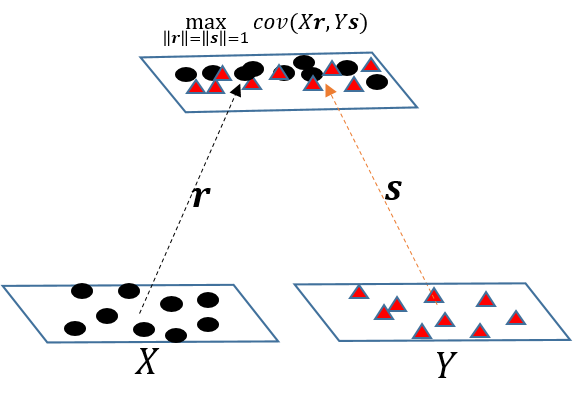
\includegraphics[width=0.5\linewidth]{source/PLS_Euclidean.png}
  	\caption{欧氏空间偏最小二乘回归示意图}
  	\label{fig:PLS_Euclidean}
\end{figure}

最后,这里简单介绍PLS与CCA的关系,更多的关于PLS,PCA,CCA之间的关系可以从\cite{pls_PLSALL}中获得;CCA与PLS作为多元统计分析中的有力工具,广泛应用于统计分析,机器学习,计算机视觉等领域;两者虽然名字差别很大但是形式上却很相近的,以至于在一些情况下可以说两者就是等价的;它们的相似性从它们的数学形式就可以看出来:
\begin{equation}
\label{pls_CCA_VS_PLS}
\begin{split}
&CCA~~:~~\max_{\|\bm{r}\|=\|\bm{s}\|=1}[corr(X\bm{r},Y\bm{s})]^2\\
&PLS~~:~~\max_{\|\bm{r}\|=\|\bm{s}\|=1}[cov(X\bm{r},Y\bm{s})]^2
\end{split}
\end{equation}
上两式的联系,在1976年H. D. Vinod关于canonical ridge analysis的论文\cite{pls_Canonical_ridge}中给出的公式\ref{pls_PCA_CCA_PLS}即可看出一二。
\begin{equation}
\label{pls_PCA_CCA_PLS}
\begin{split}
\max_{\|\bm{r}\|=\|\bm{s}\|=1}\frac{cov(X\bm{r},Y\bm{s})}{([1-\gamma_X]var(X\bm{r})+\gamma_X)([1-\gamma_Y]var(Y\bm{s})+\gamma_Y)}
\end{split}
\end{equation}
其中$0\leq \gamma_X,\gamma_Y \leq 1$,进一步的上述问题的解对应于如下特征值问题:
\begin{equation}
\label{pls_eigenproblem}
([1-\gamma_X]\bm{X^{T}X}+\gamma_X\bm{I})^{-1}\bm{X^{T}Y}([1-\gamma_Y]\bm{Y^{T}Y}+\gamma_Y\bm{I})^{-1}\bm{Y^{T}Xw}=\lambda\bm{w}
\end{equation}
总结上述内容得到:CCA与PLS与在数学形式上很相似,其中PLS最大化的是投影后的向量间的协方差,而CCA最大化的是投影后样本表示的相关系数,两者相差了一个尺度因子,在尺度因子(投影后的标准差)为1的时候两者相等;此外两者本质上都是特征值问题,且特征值问题的一般形式如式\ref{pls_eigenproblem}所示。

\section{黎曼流形上的投影问题}
\label{sec:manifold_projection}
简单回顾欧氏空间中的PCA,CCA和PLS不难发现其中都涉及到投影(如投影向量或投影矩阵)的概念,它是这一类方法的核心,也是本节的主要讨论的对象。这一节的内容主要分为两部分:第一部分从欧氏空间中的投影开始,逐步介绍抽象的投影的概念,然后将这个概念推广到黎曼流形;第二部分会具体的以SPD矩阵流形为例,将黎曼流形的投影的概念具体化。
\subsection{一般化的投影}
\label{sec:common_projection}
这里的投影理解为欧氏空间中高维空间向低维空间的投影的一般化,此外由于PCA,CCA以及PLS中的概念是相似的所以这里就直接以PLS为载体进行欧氏空间中的投影的概念的解释和一般化介绍。

\ref{sec:plsr}节给出了欧氏空间中的偏最小二乘的目标函数的形式是公式\ref{pls_max_cov},也就是最大化协方差的目标。
\begin{equation}
\label{pls_data_MaxCov}
\begin{split}
\max_{\|\bm{r}\|=\|\bm{s}\|=1}[cov(X\bm{r},Y\bm{s})]^{2}&=\max_{\|\bm{r}\|=\|\bm{s}\|=1}\left\{\sum_{i=1}^{n}(\bm{x}_{i}^{T}\bm{r}-\bar{\bm{x}}^{T}\bm{r})(\bm{y}_{i}^{T}\bm{s}-\bar{\bm{y}}^{T}\bm{s})\right\}^2\\
&=\max_{\|\bm{r}\|=\|\bm{s}\|=1}\left\{\sum_{i=1}^{n}[\bm{r}^{T}(\bm{x}_{i}-\bar{\bm{x}})][\bm{s}^{T}(\bm{y}_{i}-\bar{\bm{y}})]\right\}^2\\
\end{split}
\end{equation}
在公式\ref{pls_data_MaxCov}中$\bm{r}^{T}(\bm{x}_{i}-\bar{\bm{x}})$和$\bm{s}^{T}(\bm{y}_{i}-\bar{\bm{y}}),i=1,2,...,n$即为高维空间向低维空间的投影变换。但是这样的概念并不能很好的泛化到流形,因为流形并没有内积的定义。为此,这里先回顾一下欧氏空间中投影的更一般的形式。

高维空间向低位空间的投影的物理意义是在低维空间中找到高维空间中的原始数据最接近的表示。设$\bm{x} \in \mathbb{R}^{n}$是$n$维空间中的向量,又有$S_k$表示$n$维空间中的一个$k$维子空间,那么$\bm{x}$向$S_k$中的投影可以由如\ref{projection}所示的优化问题得到(其中$d(\cdot,\cdot)$表示的是距离函数)。
\begin{equation}
\label{projection}
\begin{split}
\Pi_{S_k}(\bm{x})=\min_{\bm{x}^{\prime} \in S_k}d^{2}(\bm{x}^{\prime},\bm{x})
\end{split}
\end{equation}
特别地,若$S_k$是一维子空间,即$S_k$是由一个向量张成的子空间$S_1=\{\bm{v}|\bm{v}=t\bm{w},t\in \mathbb{R}\text{ and }\bm{w}\in\mathbb{R}^{n}\}$,则投影变换定义如\ref{onedim_projection}所示。
\begin{equation}
\label{onedim_projection}
\begin{split}
&\Pi_{S_1}(\bm{x})=\min_{\bm{x}^{\prime} \in S_1}d^{2}(\bm{x}^{\prime},\bm{x})\\
&t^{*} \triangleq \pi_{S_1}(\bm{x})=\min_{t\in\mathbb{R}}d^{2}(t\bm{w},\bm{x})
\end{split}
\end{equation}
这里的$t$称为投影系数,也就是\ref{pls_data_MaxCov}中的$r^{T}(x_{i}-\bar{\bm{x}})$或$s^{T}(y_{i}-\bar{\bm{y}}),i=1,2,...,N$,因而\ref{pls_data_MaxCov}的问题在这个投影描述下,变成了寻找合适的一维子空间$S_{1}^{x}=\{\bm{v}|\bm{v}=t\bm{r},t\in \mathbb{R}\text{ and }\bm{r}\in\mathbb{R}^{n},\|\bm{r}\|=1\}$,$S_{1}^{y}=\{\bm{v}|\bm{v}=u\bm{s},u\in \mathbb{R}~~{\rm and}~~s\in\mathbb{R}^{n},\|\bm{s}\|=1\}$使得投影后的数据表示具有最大的协方差。
\subsection{对称正定矩阵流形上的均值}
\label{sec:riemannian_mean}
本节将就SPD矩阵流形为例,介绍其上的投影变换;此外总结欧氏空间中的PLS方法,不难发现,若要将PLS推广到黎曼流形需要完成四件事:1)数据的中心化;2)寻找合适的子流形,3)将高维空间中的数据投影到子流形中;4)最大化的协方差。本节的内容主要完成的是前两件事:数据的中心化和寻找合适的子流形。由于子流形的构造与中心化相关,所以本节先花一点篇幅简要回顾SPD上的Karcher mean问题。

由于在本文的第二章中,针对该问题已有详细的的介绍和讨论,所以这里我们直接给出它计算的数学形式。
\begin{displaymath}
\bar{\bm{x}}=\min_x\frac{1}{2n}\sum_{i=1}^{n}\delta^{2}(\bm{x},\bm{x}_i)
\end{displaymath}
这里的$\delta(\cdot,\cdot)$表示的是流形中的测地距离,在PSD流形中常使用也是最基本的就是仿射不便距离(Affine Invariant Distance,AID)\cite{AIM_metric},将AID带入到上式的话得到:
\begin{equation}
\label{AIM_mean}
\begin{split}
\mu&=\min_{X}f(X)=\min_{X}\frac{1}{2n}\sum_{i=1}^{n}\delta^{2}(X,X_i)\\
&=\min_{X}\frac{1}{2n}\sum_{i=1}^{n}\|\log(X^{-\frac{1}{2}}X_iX^{-\frac{1}{2}})\|_F
\end{split}
\end{equation}
其中,由于使用$\mu$来表示样本均值已经是约定俗成的了所以尽管Karcher mean是一个矩阵,这里仍然用$\mu$来表示。第二章已经介绍过要想求出公式\ref{AIM_mean}的解析解几乎是不可能的,但是作为优化问题的话,优化算法仍然是可用的,因此主要的问题就是计算公式\ref{AIM_mean}的梯度函数,在第二章中我们有如下的结果:
\begin{equation}
\label{AIM_grad}
\begin{split}
{\rm dist}(X,X_i)&=\|\log(X^{-\frac{1}{2}} X_i X^{-\frac{1}{2}})\|_{F},i=1,2,...,n\\
\nabla_X {\rm dist}(X,X_i)&=2X^{\frac{1}{2}}\log(X^{\frac{1}{2}}X_{i}^{-1}X^{\frac{1}{2}})X^{\frac{1}{2}}=-2\log_{X}(X_i)
\end{split}
\end{equation}
将上式带入到\ref{AIM_mean}得到:
\begin{equation}
\label{AIM_mean_grad}
\begin{split}
\nabla f(X)&=\frac{1}{2n}\sum_{i=1}^{n}2X^{\frac{1}{2}}\log(X^{\frac{1}{2}}X_{i}^{-1}X^{\frac{1}{2}})X^{\frac{1}{2}}\\
&=-\frac{1}{n}\sum_{i=1}^{n}\log_{X}(X_i)
\end{split}
\end{equation}
利用\ref{AIM_mean_grad}不难得到黎曼流形上的梯度下降更新公式(其中$k$是迭代次数,$\tau$代表步长)。
\begin{equation}
\label{AIM_grad_update}
\mu_{k+1}=\exp_{\mu_k}(\frac{\tau}{n}\sum_{i=1}^{n}\log_{\mu_k}(X_i))
\end{equation}
\subsection{黎曼流形上的子流形与投影}
\label{sec:riemannian_mean}
在\ref{sec:riemannian_mean}节介绍了黎曼流形上的均值的计算,这节将会介绍黎曼流形上高维流形向低维流形的投影的过程,此前在文献\cite{PGA,RCCA}中对该问题就有一些介绍,这里会对之前工作做一个总结,为黎曼流形上的PLS推广做准备。

首先,根据欧氏空间中的高维空间向一维子空间的投影形式(公式\ref{onedim_projection}),可以看出确定一个一维的子流形是投影变换的首要任务,并注意到流形上的测地线是链接两点之间最短的曲线,它是欧氏空间中两点之间直线最短的概念的推广,因此利用测地线构造子流形是自然的一种途径,而从流形上的均值(Karcher mean)出发的测地线常用于构造这样的子流形(目前还没有理论证明这样的构造是最优的,但是一部分在PSD流形上的实验结果验证了在均值这点可以得到不错的结果\cite{RegionCov_pedestrain}),于是将从Karcher mean出发利用测地线构造子空间记为$S_W$,带入到公式\ref{onedim_projection}中并使用测第距离可得到公式\ref{submanifold_projection}的形式。
\begin{equation}
\label{submanifold_projection}
\begin{split}
\Pi_{S_W}(X)=\min_{X^{\prime} \in S_W}\delta^{2}(X^{\prime},X)
\end{split}
\end{equation}
更具体地,当把上述理论运用到对称正定矩阵流形的时候(使用Affine Invariant Distance\cite{AIM_metric}),可以更具体的得到公式\ref{SPD_submanifold}的形式。
\begin{equation}
\label{SPD_submanifold}
\left\{
\begin{split}
\begin{aligned}
&S_W=\exp_\mu({\rm{span}}(W)\cap U)\\
&\Pi_{S_W}(X)=\min_{X^{\prime} \in S_W}\delta^{2}(X^{\prime},X)\\
&~~~~~~~~~~=\min_{t \in (-\epsilon,\epsilon),X^{\prime}=tW}\|\log_{[\exp_{\mu}(tW)]}(X)\|^2\\
&\pi_{S_W}(X)=\min_{t \in (-\epsilon,\epsilon)}\|\log_{[\exp_{\mu}(tw)]}(X)\|^2=t^{*}
\end{aligned}
\end{split}
\right.
\end{equation}
其中$W$就是Karcher mean的切空间中从原点出发的一条切向量,类似于欧氏空间中数据中心化后的空间中的投影方向;公式\ref{SPD_submanifold}即包含了子流形的构造以及原始流形向子流形的投影。为了方便理解这里使用示意图\ref{fig:SPD_SubManifold}
帮助理解。
\begin{figure}
	\centering
	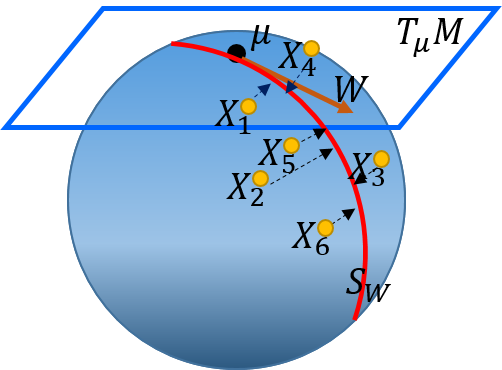
\includegraphics[width=0.5\linewidth]{source/SPD_submanifold.png}
	\caption{流形上的投影示意图}
	\label{fig:SPD_SubManifold}
\end{figure}
\section{黎曼流形上的偏最小二乘回归问题}
\label{sec:RPLS}
本节将借助前面定义的子流形和投影的概念对SPD矩阵流形的一般形式化进行阐述,然后在接下来的一小节中,将结合这种一般化形式针对图像集合分类问题的特点,对其做进一步的改进,使其更加适配到图像集合分类问题上。
\subsection{黎曼流形上偏最小二乘回归问题的一般形式}
\label{sec:RPLS_common}
首先是黎曼流形上的偏最小二乘问题:假设$\{X_i\}_{i=1}^{n},\{Y_i\}_{i=1}^{n} \subset M$是来自对称正定矩阵流形$M$的两组样本,根据公式\ref{submanifold_projection}以及公式\ref{pls_data_MaxCov}这里可以写出如下的目标函数:
\begin{equation}
\label{Riemannian_PLS}
\begin{split}
\max_{w_x,w_y}& C^2(w_x,w_y)=\max_{w_x,w_y}{\left(\sum_{i=1}^{n}(t_i-\bar{t})(u_i-\bar{u})\right)^2}\\
s.t.~~&t_i=\min_{X(t) \in S_{w_x},t \in (-\epsilon,\epsilon)}\delta^{2}(X(t),X_i);i=1,2,..,n;\\
&u_i=\min_{Y(u) \in S_{w_y},u \in (-\eta,\eta)}\delta^{2}(Y(u),Y_i);i=1,2,...,n;\\
&\|w_x\|=\|w_y\|=1;\bar{t}=\frac{1}{n}\sum_{i=1}^{n}t_i;\bar{u}=\frac{1}{n}\sum_{i=1}^{n}u_i.
\end{split}
\end{equation}
将上述的形式化具体到SPD矩阵流形:假设$\{X_i\}_{i=1}^{n},\{Y_i\}_{i=1}^{n} \subset \mathbb{S}_{d}^{+}$是来自对称正定矩阵流形$\mathbb{S}_{d}^{+}$的两组样本,根据公式\ref{SPD_submanifold}以及公式\ref{pls_data_MaxCov}这里可以写出如下的目标函数:
\begin{equation}
\label{SPD_RPLS}
\begin{split}
\max_{W_X,W_Y}& C^2(W_X,W_Y)=\max_{W_X,W_Y}{\left(\sum_{i=1}^{n}(t_i-\bar{t})(u_i-\bar{u})\right)^2}\\
s.t.~~&t_i=\min_{t \in (-\epsilon,\epsilon)}\|\log_{[\exp_{\mu_x}(tW_X)]}(X_i)\|^2;i=1,2,..,n;\\
&u_i=\min_{u \in (-\eta,\eta)}\|\log_{[\exp_{\mu_y}(uW_Y)]}(Y_i)\|^2;i=1,2,...,n;\\
&\|W_X\|=\|W_Y\|=1;\bar{t}=\frac{1}{n}\sum_{i=1}^{n}t_i;\bar{u}=\frac{1}{n}\sum_{i=1}^{n}u_i.
\end{split}
\end{equation}

公式\ref{SPD_RPLS}描述了SPD矩阵流形上的偏最小二乘问题的一般形式,也是定义了流形中的投影之后所能得到的最直接的形式化;但是不难发现还有如下一些问题遗留:1)由于公式\ref{SPD_RPLS}没有解析解,上述问题需要大量的计算,消耗时间过长是一个问题,究其原因主要是$t_i=\min_{t \in (-\epsilon,\epsilon)}\|\log_{[\exp_{\mu_x}(tW_X)]}(X_i)\|^2;i=1,2,..,n;$和$u_i=\min_{u \in (-\eta,\eta)}\|\log_{[\exp_{\mu_y}(uW_Y)]}(Y_i)\|^2;i=1,2,...,n;$的计算过于复杂。2)如何像欧氏空间中的PLS一般计算第二个(或更多个)投影方向(子空间);3)如何将上述问题用于分类问题(或者说如何做回归问题)。在接下来的内容我们将会发现:这些问题中最主要的问题还是原问题没有解析解的问题,当通过适当近似手段将原问题简化后,上面列出的几个问题都将迎刃而解。

前面已经提到优化问题\ref{SPD_RPLS}的计算复杂度过高,并且该问题在图像集合分类问题上会更加严重,原因是数据的维度太高,所以这里选择适当的近似以求在保证一定的精度的同时速度能有较大的提升。

这里的近似的方法在工作\cite{RCCA,PGA}中已有类似的介绍,主要的思想就是针对$t_i=\min_{t \in (-\epsilon,\epsilon)}\|\log_{[\exp_{\mu_x}(tW_X)]}(X_i)\|^2;i=1,2,..,n;$和$u_i=\min_{u \in (-\eta,\eta)}\|\log_{[\exp_{\mu_y}(uW_Y)]}(Y_i)\|^2;i=1,2,...,n;$的计算复杂过高(或者说没有解析解)的问题而提出的简化方案。

以$t_i=\min_{t \in (-\epsilon,\epsilon)}\|\log_{[\exp_{\mu_x}(tW_X)]}(X_i)\|^2$为例,这里我们不难发现时间复杂度主要来自于$\|\log_{[\exp_{\mu_x}(tW_X)]}(X_i)\|^2$而这一部分实际上描述了这样一个过程:将Karcher mean($\mu_x$)的切空间中的向量$tW_X$通过$\exp_{\mu_x}(\cdot)$变换到$\mathbb{S}_{d}^{+}$中然后在$\mathbb{S}_{d}^{+}$中度量$\exp_{\mu_x}(tW_X),X_i$两者的测地距离$\delta(\exp_{\mu_x}(tW_X),X_i)$;据此我们使用如下的近似方案(具体的参考\cite{PGA}),将在原流形中度量$\exp_{\mu_x}(tW_X),X_i$两者的距离改用在$\mu_x$的切空间中度量两者的距离${\rm dist}(\exp_{\mu_x}(tW_X),X_i)\approx \|tW_X-\log_{\mu_x}(X_i)\|_{\mu_x}$,于是原来的投影问题\ref{SPD_submanifold}就变成了:
\begin{equation}
\label{tangent_approxiamte}
\Pi_{S}(X)=\exp\left(\mu_x,\sum_{i=1}^{k}V_i\left<V_i,\log_{\mu_x}(X)\right>\right)\\
\end{equation}
其中$\{V_i\}_{i=1}^{d}$是$\mu_x$处的切空间中的标准正交基($\mu_x$的切空间是内积空间),这点修改使得问题大大简化,稍作整理之后我们可以得到的算法\ref{alg:RPLS_approx}中的对称正定矩阵流形上的偏最小二乘近似算法。
\begin{algorithm}[htb]
\caption{对称正定矩阵流形上的偏最小二乘近似算法}
\label{alg:RPLS_approx}
\begin{algorithmic}[1]
\REQUIRE 对称正定矩阵集合$\bm{X}=\{X_i\}_{i=1}^{n},\bm{Y}=\{Y_i\}_{i=1}^{n}$,需要计算的成分的个数$k$
\ENSURE 在集合$\bm{X}$的Karcher mean($\mu_x$)处的切空间中张成子空间的$k$个成分$\bm{W}_{X}=\{W_{X}^{i}\}_{i=1}^{k}$,以及$\{X_i\}_{i=1}^{n}$对应的投影$\{\bm{t}_i\}_{i=1}^{n}$;在集合$\bm{Y}$的Karcher mean($\mu_y$)处的切空间中张成子空间的$k$个成分$\bm{W}_{Y}=\{W_{Y}^{i}\}_{i=1}^{k}$,以及$\{Y_i\}_{i=1}^{n}$对应的投影$\{\bm{u}_i\}_{i=1}^{n}$;
\STATE 计算$\mu_x, \mu_y$和$\{\hat{X}_i=\log_{\mu_{x}}(X_i)\}_{i=1}^{n}, \{\hat{Y}_i=\log_{\mu_{y}}(Y_i)\}_{i=1}^{n}$
\STATE 利用群操作将样本变换到单位矩阵的切空间:\\
~~~~~~~~~~~~~~~~~~~$\log_{\mu_{x}}(X_i)\rightarrow \mu_{x}^{-1/2}\log_{\mu_{x}}(X_i)\mu_{x}^{-1/2}=\log(\mu_{x}^{-1/2}X_i\mu_{x}^{-1/2})\triangleq \tilde{X}_i$\\
~~~~~~~~~~~~~~~~~~~$\log_{\mu_{y}}(Y_i)\rightarrow \mu_{y}^{-1/2}\log_{\mu_{y}}(Y_i)\mu_{y}^{-1/2}=\log(\mu_{y}^{-1/2}Y_i\mu_{y}^{-1/2})\triangleq \tilde{Y}_i$
\STATE 在$\{\tilde{X}_{i}\}_{i=1}^{n}$以及$\{\tilde{Y}_{i}\}_{i=1}^{n}$之间执行PLS得到$\hat{\bm{W}}_X,\hat{\bm{W}}_Y,T=[\bm{t}_1,\cdots,\bm{t}_k],U=[\bm{u}_1,\cdots,\bm{u}_n]$
\STATE 利用群操作将$\hat{\bm{W}}_X$变换到$\mu_x$的切空间得到$\bm{W}_X$,将$\hat{\bm{W}}_y$变换到$\mu_y$的切空间得到$\bm{W}_Y$
\RETURN $\bm{W}_X,\bm{W}_Y,T,U$
\end{algorithmic}
\end{algorithm}

算法\ref{alg:RPLS_approx}中的:\textit{“在$\{\tilde{X}_{i}\}_{i=1}^{n}$以及$\{\tilde{Y}_{i}\}_{i=1}^{n}$之间执行PLS得到$\hat{\bm{W}}_X,\hat{\bm{W}}_Y,T=[\bm{t}_1,\cdots,\bm{t}_k],U=[\bm{u}_1,\cdots,\bm{u}_n]$”}使用的是欧氏空间中的标准的PLS问题,因为Karcher mean的切空间是内积空间,而通过群操作后的数据在单位阵$I$处的表示也是内积空间,所以欧氏空间中的方法在这里都可以直接使用,进一步的,通过公式\ref{pls_score_model}$\sim$\ref{label_represent}的内容即可得到计算多个成分(投影子空间)和PLS做回归问题的形式化,由于这只是重复前面的内容,这里就不再赘述了,最后在\ref{alg:RPLS_approx_regression}中给出与算法\ref{alg:RPLS_approx}类似的用于回归问题的算法。
\begin{algorithm}[hbt]
\caption{对称正定矩阵流形上的偏最小二乘回归近似算法}
\label{alg:RPLS_approx_regression}
\begin{algorithmic}[1]
\REQUIRE 对称正定矩阵集合$\bm{X}=\{X_i\}_{i=1}^{n}$,label矩阵$Y$,需要计算的成分的个数$k$
\ENSURE 在集合的$\bm{X}$的Karcher mean($\mu$)处的切空间处张成子流形的$k$个成分$\bm{W}_{X}=\{W_{X}^{i}\}_{i=1}^{k}$,以及$\{X_i\}_{i=1}^{n}$对应的投影$\{\bm{t}_i\}_{i=1}^{n}$;欧氏空间中标签集$Y$的投影向量$W_y=\{w_{y}^{i}\}_{i=1}^{k}$及其对应的投影$\{\bm{u}_i\}_{i=1}^{n}$
\STATE 计算$\bm{X}$的Karcher mean($\mu$)以及$\{\hat{X}_i=\log_{\mu}(X_i)\}_{i=1}^{n}$
\STATE 利用群操作将样本移动到单位矩阵的切空间:\\
 ~~~~~~~~~~~~~~~~~~~~$\log_{\mu}(X_i)\rightarrow \mu^{-1/2}\log_{\mu}(X_i)\mu^{-1/2}=\log(\mu^{-1/2}X_i\mu^{-1/2})\triangleq \tilde{X}_i$
\STATE 在$\{\tilde{X}_{i}\}_{i=1}^{n}$以及$Y$之间执行PLS回归得到$\hat{\bm{W}}_x,W_y,T=[\bm{t}_1,\cdots,\bm{t}_k],U=[\bm{u}_1,\cdots,\bm{u}_n]$
\STATE 利用群操作将$\hat{\bm{W}}_x$变换到$\mu$的切空间得到$\bm{W}_x$
\RETURN $\bm{W}_X,W_y,T,U$
\end{algorithmic}
\end{algorithm}
\subsection{面向图像集合分类的黎曼流形上的篇最小二乘回归}
\label{sec:ImageSet_PLS}
这里将算法\ref{alg:RPLS_approx_regression}算法称为基础版本的黎曼流形上的PLS回归,该算法已经可以直接运用到图像集合分类问题了,但是仔细回顾公式\ref{Riemannian_PLS},会发现在计算$t_i,u_i$的时候要求$t_i \in (-\epsilon,\epsilon),u_i \in (-\eta,\eta)$,也就是要求$t_iW_X,u_iW_Y$在$\mu_x,\mu_y$的一个小邻域内,而其本质上是要求SPD矩阵样本的分布是比较集中;这也正是图像集合问题和DTI图像中的Tensor的重要区别之一(图像集合中的样本由于维度高样本少,所以分布往往比较稀疏),也是将黎曼流形上的PLS回归用到图像集合需要解决的问题;此外注意到工作\cite{RCCA,PGA}利用Karcher mean的切空间构造子流形,但是前面已经提到并没有理论证明这样的结果是最好的,所以如果在构造子流形的过程中考虑label的信息相信可以找到更适合构建子流形的地方。接下来的内容是如何针对以上的问题将PLS方法适配到图像集合分类上,并且我们尽量做到在几乎不增加计算复杂度的前提下方法对分类问题的解决有较大的改进。
\subsubsection{融合判别信息的子流形构造}
\label{sec:discrim_single_support}
本节将针对前面提到的第二个问题:找到一个比Karcher mean更具有一定判别性的点构建子流形的我们的解决方案进行说明。具体方案如下,首先注意到公式\ref{AIM_mean}计算Karcher mean的时候是一个无监督的优化过程,所以并未编码判别信息在其中;因此这里考虑编码label到构造子流形的点(相当于算法\ref{alg:RPLS_approx_regression}中的$\mu$),这里为方便起见仍然沿用记号$\mu$。

该步骤的目标是使得在\ref{alg:RPLS_approx_regression}中的$\{X_i\}_{i=1}^{n}$在$\mu$处的切向量表示经过群操作变换到单位阵的切空间中之后的$\{\tilde{X}_i\}_{i=1}^{n}$同类相似度大,异类相似度小,在实际中使用的是cosine相似度,也就是同类的尽量共线,不同类的尽量正交,并保证投影之后“方差”尽量的小(类似于中心化,因为直接进行中心化比较困难,所以在优化的过程要求$\{X_i\}_{i=1}^{n}$在$\mu$处的切向量表示在原切空间($T_{\mu}M$)中应该具有0均值的特点。

沿用之前的记号设$\{X_i\}_{i=1}^{n}$是来自于$C$个类的对称正定矩阵的样本$X_i \in \mathbb{S}_{d}^{+}$,并假设每个类有$n_i,i=1,2,\cdots,C$个样本$n=\sum_{i=1}^{C}n_i$,样本的label我们用公式\ref{label_represent}的矩阵$Y$表示,下面是编码判别信息的形式化过程。
\begin{itemize}
\item 定义平方相似度矩阵$F=[\rho_{ij}^{2}]_{n\times n},\rho_{ij}=\frac{k_{ij}}{\sqrt{k_{ii}k_{jj}}}$,其中$k_{ij}$由下式定义:
\begin{equation}
\begin{split}
k_{ij}&=\left<\tilde{X}_i,\tilde{X}_j\right>\\
&=\left<\log(\mu^{-1/2}X_i\mu^{-1/2}),\log(\mu^{-1/2}X_j\mu^{-1/2})\right>\\
&=\left<\log(\mu^{1/2}X_{i}^{-1}\mu^{1/2}),\log(\mu^{1/2}X_{j}^{-1}\mu^{1/2})\right>\\
\end{split}
\end{equation}
\item 定义矩阵$P^{\prime}=1-2YY^{T}$,进一步的为了平衡正负样本对之间($P^{\prime}$中的1的个数和-1的个数)的比例,这里做一下平衡操作:设$n_{\#1}$=\{$P^{\prime}$中1的个数\},$n_{\#-1}$=\{$P^{\prime}$中-1的个数\}则定义平衡后的矩阵为$P$,其中:
\begin{equation}
P_{ij}=\left\{
\begin{split}
&\frac{P_{ij}^{\prime}}{n_{\#1}},if~~P_{ij}^{\prime}=1\\
&\frac{P_{ij}^{\prime}}{n_{\#-1}},if~~P_{ij}^{\prime}=-1
\end{split}
\right.
\end{equation}
\item 根据工作\cite{PGA},这里定义“方差”:$\frac{1}{n}\sum_{i=1}^{n} \|\log_{\mu}(X_i)\|^2$
\item 最后的目标函数为:
\begin{equation}
\label{support_search}
\min_{\mu}f(\mu)={\rm tr}(FP^{T})+\frac{\lambda}{n}\sum_{i=1}^{n} \|\log_{\mu}(X_i)\|^2,\mu \succ 0
\end{equation}
其中$\lambda$是一个平衡因子起到平衡两者权重的作用,同时也有平衡量纲的作用,避免其中一方因量纲问题绝对占优。
\end{itemize}
\subsubsection{融合判别信息的切空间构造问题的优化}
\label{sec:discrim_single_support_opt}
公式\ref{support_search}没有解析解因此需要通过需要通过优化来求解,而且约束条件$\mu \succ 0$表明了问题的解空间是$\mathbb{S}_{d}^{+}$,这里我们使用黎曼流形上的共轭梯度算法(conjugate gradient methods\ref{alg:Manifold_Gradient_Descend})来优化问题\ref{support_search},关于黎曼流形上的共轭梯度算法可以参看本文的第二章以及文献\cite{Conjugate_Gradient_Survery},使用该方法优化的时候,最主要的输入就是\ref{support_search}的导数。接下来将利用第二章的内容对公式\ref{support_search}的导数计算作简要说明。

公式\ref{support_search}主要包含两部分:${\rm tr}(FP^{T})$和$\frac{\lambda}{n}\sum_{i=1}^{n} \|\log_{\mu}(X_i)\|^2$;这里先对第一部分的导数进行计算:
\begin{equation}
\label{support_search_part1_gradeint}
\begin{split}
{\rm tr}(FP^{T})&=\sum_{i=1}^{n}\sum_{j=1}^{n}F_{ij}P_{ij}=\sum_{i=1}^{n}\sum_{j=1}^{n}P_{ij}\frac{k_{ij}^2}{k_{ii}k_{jj}}\\
\frac{\partial}{\partial \mu}{\rm tr}(FP^{T})&=\sum_{i=1}^{n}\sum_{j=1}^{n}P_{ij}\left(c_1\frac{\partial}{\partial \mu}k_{ij}-c_2\frac{\partial}{\partial \mu}k_{ii}-c_3\frac{\partial}{\partial \mu}k_{jj}\right)\\
{\rm where~~}c_1&=\frac{2k_{ij}k_{ii}k_{jj}}{(k_{ii}k_{jj})^2},c_2=\frac{k_{ij}k_{ij}k_{jj}}{(k_{ii}k_{jj})^2},c_3=\frac{k_{ij}k_{ij}k_{ii}}{(k_{ii}k_{jj})^2}
\end{split}
\end{equation}
公式\ref{support_search_part1_gradeint}表明导数的计算的核心主要是$\frac{\partial}{\partial \mu}k_{ij}$,因此剩下的工作主要就是$k_{ij}$的导数计算;在此之前这里先对$k_{ij}$的形式稍加变换,这样会比较方便理解后面的$k_{ij}$的导数的形式(公式\ref{kernel_elementwise_gradient}):
\begin{equation}
\label{kernel_elementwise}
\begin{split}
&\left<\log_{\mu}(X_i),\log_{\mu}(X_j)\right>_{\mu}\\
&~~~~~~=\left<\log(\mu^{-1/2}X_{i}\mu^{-1/2}),\log(\mu^{-1/2}X_j\mu^{-1/2})\right>\\
&~~~~~~=\left<\log(\mu^{1/2}X_{i}^{-1}\mu^{1/2}),\log(\mu^{1/2}X_{j}^{-1}\mu^{1/2})\right>\\
&~~~~~~={\rm tr}(\log(X_{i}^{-1}\mu)\log(X_{j}^{-1}\mu))\\
&~~~~~~={\rm tr}(X_{i}^{-1/2}\log(X_{i}^{-1/2}\mu X_{i}^{-1/2})X_{i}^{1/2}X_{j}^{-1/2}\log(X_{j}^{-1/2}\mu X_{j}^{-1/2})X_{j}^{1/2})\\
&~~~~~~={\rm tr}(\log(X_{i}^{-1/2}\mu X_{i}^{-1/2})X_{i}^{1/2}X_{j}^{-1/2}\log(X_{j}^{-1/2}\mu X_{j}^{-1/2})X_{j}^{1/2}X_{i}^{-1/2})\\
&~~~~~~=\left<\log(X_{i}^{-1/2}\mu X_{i}^{-1/2}),X_{i}^{1/2}X_{j}^{-1/2}\log(X_{j}^{-1/2}\mu X_{j}^{-1/2})X_{j}^{1/2}X_{i}^{-1/2}\right>\\
\end{split}
\end{equation}
下面给出$k_{ij}$的导数的具体形式,由于比较复杂,感兴趣的读者可以参看本文第二章以及文献\cite{Maniopt_DiscreteCurveFitting,Statistics_SLEDML}的相关章节。
\begin{equation}
\label{kernel_elementwise_gradient}
\begin{split}
&\frac{\partial}{\partial \mu}k_{ij}=X_{i}^{-1/2}\left(D\log(X_{i}^{-1/2}\mu X_{i}^{-1/2})[sym(X_{i}^{1/2}X_{j}^{-1/2}\log(X_{j}^{-1/2}\mu X_{j}^{-1/2})X_{j}^{1/2}X_{i}^{-1/2}]\right)X_{i}^{-1/2}\\
&~~~~~~+X_{j}^{-1/2}\left(D\log(X_{j}^{-1/2}\mu X_{j}^{-1/2})[sym(X_{j}^{1/2}X_{i}^{-1/2}\log(X_{i}^{-1/2}\mu X_{i}^{-1/2})X_{i}^{1/2}X_{j}^{-1/2}]\right)X_{j}^{-1/2}\\
\end{split}
\end{equation}

至于第二部分的$\frac{\lambda}{n}\sum_{i=1}^{n} \|\log_{\mu}(X_i)\|^2$的导数,不难发现以下的关系$\|\log_{\mu}(X_i)\|^2=\left<\log_{\mu}(X_i),\log_{\mu}(X_i)\right>_{\mu}=k_{ii}$,因此这部分的导数可以根据\ref{kernel_elementwise_gradient}直接导出来。
\begin{equation}
\label{support_search_part2_gradeint}
\begin{split}
\frac{\partial}{\partial \mu}\frac{\lambda}{n}\sum_{i=1}^{n} \|\log_{\mu}(X_i)\|^2=\frac{\lambda}{n}\sum_{i=1}^{n}\frac{\partial}{\partial \mu}k_{ii}
\end{split}
\end{equation}
整合两部分的结果可以得到公式\ref{support_search}在普通欧氏空间中关于$\mu$的导数如公式\ref{support_search_gradeint}所示。
\begin{equation}
\label{support_search_gradeint}
\nabla_{\mu} f(\mu)=\sum_{i=1}^{n}\sum_{j=1}^{n}P_{ij}\left(c_1\frac{\partial}{\partial \mu}k_{ij}-c_2\frac{\partial}{\partial \mu}k_{ii}-c_3\frac{\partial}{\partial \mu}k_{jj}\right)+\frac{\lambda}{n}\sum_{i=1}^{n}\frac{\partial}{\partial \mu}k_{ii}
\end{equation}
最后,利用第二章中的内容以及论文\cite{Statistics_SLEDML,Maniopt_DiscreteCurveFitting}中的结果将普通的梯度转换为黎曼梯度。这只需要对公式\ref{support_search_gradeint}作公式\ref{support_search_riemannian_gradeint}中的变化即可:
\begin{equation}
\label{support_search_riemannian_gradeint}
{\rm grad}_{\mu}f(\mu)=\mu \nabla_{\mu} f(\mu) \mu
\end{equation}
将优化公式\ref{support_search}得到的$\mu$代替算法\ref{alg:RPLS_approx_regression}中的Karcher mean并在该点做投影变化,即得到了融入判别信息的改进方法;虽然目前的结果不是本文所提算法的最终形式,但是这是最终算法的基础,在后面的章节中将会反复使用到,所以这里将其总结在算法\ref{alg:RPLS_discrim_tangent_approx_regression}中。
\begin{algorithm}
\caption{对称正定矩阵流形上具有判别性的切空间偏最小二乘回归近似算法}
\label{alg:RPLS_discrim_tangent_approx_regression}
\begin{algorithmic}[1]
\REQUIRE 对称正定矩阵集合$\bm{X}=\{X_i\}_{i=1}^{n}$,label矩阵${Y}$,需要计算的成分的个数$k$
\ENSURE 融入判别性的切空间$T_{\mu}M$对应的$\mu$,集合$\bm{X}$在$T_{\mu}M$中的$k$个成分$\bm{W}_X=\{W_{X}^{i}\}_{i=1}^{k}$,以及$\{X_i\}_{i=1}^{n}$对应的投影$\{\bm{t}_i\}_{i=1}^{n}$;欧氏空间中标签集$\bm{Y}$的投影向量$W_y=\{\bm{w}_{y}^{i}\}_{i=1}^{k}$及其对应的投影$\{\bm{u}_i\}_{i=1}^{n}$
\STATE 初始化$\mu=\mu_0$(通常为$I$)求解最小化问题2.1获得$\mu$,然后计算$\{\hat{X}_i=\log_{\mu}(X_i)\}_{i=1}^{n}$
\STATE 利用群操作将样本移动到单位矩阵的切空间:\\
 ~~~~~~~~~~~~~~~~~~~~$\log_{\mu}(X_i)\rightarrow \mu^{-1/2}\log_{\mu}(X_i)\mu^{-1/2}=\log(\mu^{-1/2}X_i\mu^{-1/2})\triangleq \tilde{X}_i$
\STATE 在$\{\tilde{X}_{i}\}_{i=1}^{n}$以及${Y}$之间执行PLS回归得到$\hat{\bm{W}}_X,W_y,T=[\bm{t}_1,\cdots,\bm{t}_k],U=[\bm{u}_1,\cdots,\bm{u}_n]$
\STATE 利用群操作将$\hat{W}_x$变换到$\mu$的切空间得到$\bm{W}_x$
\RETURN $\bm{W}_X,W_y,T,U$
\end{algorithmic}
\end{algorithm}
最后,为了方便理解\ref{alg:RPLS_discrim_tangent_approx_regression}算法这里使用利用示意图\ref{fig:discrim_tangent_RPLS}对算法的思想进行说明。
\begin{figure}
	\centering
	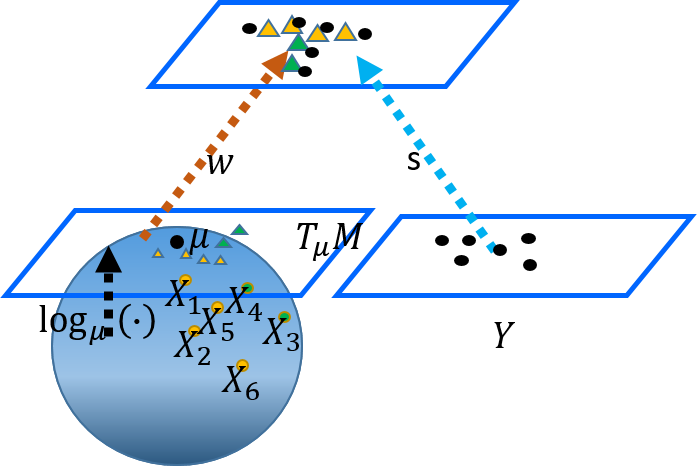
\includegraphics[width=0.5\linewidth]{source/Discrim_Tangent_PLS.png}
	\caption{算法\ref{alg:RPLS_discrim_tangent_approx_regression}的示意图}
	\label{fig:discrim_tangent_RPLS}
\end{figure}
\subsubsection{多切空间逐步回归的偏最小二乘方法}
\label{sec:muliti_tangent_rpls}
注意到算法\ref{alg:RPLS_discrim_tangent_approx_regression}仍然没有解决一开始提到的另一个问题:数据不紧凑所带来的近似/估计不准问题,接下来的部分将针对这个问题做进一步的改进。公式\ref{SPD_RPLS}中的$t_i \in (-\epsilon,\epsilon)$和$u_i \in (-\eta,\eta)$的条件就是要求样本数据需要足够集中才行,但是如果直接将算法\ref{alg:RPLS_discrim_tangent_approx_regression}中的$\bm{t}_i$或$\bm{u}_i$进行截断的话,这不仅会损失精度(因为原始数据本来分布很稀疏,再限制$t_i$或$u_i$的取值范围无疑会使得估计更加的不准),而且在优化的时候也会比较麻烦,所以这里考虑寻找多个点使用多个切空间来缓解数据稀疏的问题。在这样的框架下,每个切空间并不需要很强的表示能力,只需要能够反应原始数据的一部分结构就行,而最后通过设计特定的方法整合每个切空间中的表示模型得到更具表示能力的模型帮助判别(分类)问题的研究。

上述框架的主要问题是如何选取各个切空间以及如何将他们有效的融合起来,这里我们使用逐步回归的方案来同时解决这两个问题:对算法\ref{alg:RPLS_discrim_tangent_approx_regression}中的数据$\bm{X}=\{X_i\}_{i=1}^{n}$和label矩阵${Y}$执行算法\ref{alg:RPLS_discrim_tangent_approx_regression}得到获得一个切空间$T_{\mu_1}M$及其对应的$k$个投影方向$\bm{W}_{X}^{(1)},W_{y}^{(1)}$和对应的$T_{1},U_{1}$;然后对$\{\tilde{X}_{i=1}^{n}\}$以及$Y$利用公式\ref{pls_deflate}进行defalte操作:%$\underrightarrow{abc}$,
$\{\tilde{X}_{i}\}_{i=1}^{n} \xlongrightarrow{defalte} \{\tilde{X}^{res}_i\}_{i=1}^{n},{Y}\xlongrightarrow{defalte} {Y}^{res}$,然后对$\{\tilde{X}^{res}_{i}\}_{i=1}^{n}$利用群操作从单位阵处将数据变换到$\mu$再用$\exp_{\mu_{1}}(\cdot)$将数据$\{\tilde{X}^{res}_i\}_{i=1}^{n}$变换到SPD矩阵流形得到$\{Z^{res}_{i}\}_{i=1}^{n}$,最后将$\{Z^{res}_i\}_{i=1}^{n},{Y}^{res}$赋值给$\bm{X}=\{X_i\}_{i=1}^{n}$和$Y$,并重新初始化$\mu_2$后开始第二次迭代;反复上述过程直到获得指定个数的切空间,算法终止。将上述过程用算法\ref{alg:RPLS_multi_support_approx_regression}描述。
\begin{algorithm}[htb]
\caption{对称正定矩阵流形上多切空间偏最小二乘回归近似算法}
\label{alg:RPLS_multi_support_approx_regression}
\begin{algorithmic}[1]
\REQUIRE 对称正定矩阵集合$\bm{X}=\{X_i\}_{i=1}^{n}$,label矩阵${Y}$,每个切空间计算的成分的个数$k$,指定切空间的个数$p$
\ENSURE 融入判别性的$p$个切空间$T_{\mu_1}M,\cdots,T_{\mu_{p}}M$对应的$\mu_{1},\cdots \mu_{p}$,数据$\bm{X}$在$T_{\mu_1}M,\cdots,T_{\mu_{p}}M$中各自的$k$个成分$\bm{W}_{x}^{(1)},\cdots,\bm{W}_{x}^{(p)}$,以及对应的投影$T_1,\cdots,T_{p}$;欧氏空间中标签集${Y}$逐次回归的投影矩阵$W_{y}^{(1)},\cdots,W_{y}^{(p)}$及其对应的投影$U_1,\cdots,U_{p}$
\STATE 初始化$output$为包含$p$个cell的结构:$output=cell(1,p)$
\FOR{$j=1;~j\leq p;~j=j+1$}
	\STATE 初始化$\mu_j=\mu_0$(通常为$I$)最小化2.1问题获得$\mu_j$,然后计算$\{\hat{X}_i=\log_{\mu_j}(X_i)\}_{i=1}^{n}$
	\STATE 利用群操作将样本移动到单位矩阵的切空间:\\
 	~~~~~~~~~~~~~~~~~~~~$\log_{\mu_{j}}(X_i)\rightarrow \mu_{j}^{-1/2}\log_{\mu}(X_i)\mu_{j}^{-1/2}=\log(\mu_{j}^{-1/2}X_i\mu_{j}^{-1/2})\triangleq \tilde{X}_i$
	\STATE 在$\{\tilde{X}_{i}\}_{i=1}^{n}$以及$\bm{Y}$之间执行PLS回归得到:\\
	$\hat{\bm{W}}_{x}^{(j)},W_{y}^{(j)},T_{j}=[\bm{t}_{1}^{j},\cdots,\bm{t}_{k}^{j}],U_j=[\bm{u}_{1}^{j},\cdots,\bm{u}_{k}^{j}]$
	\STATE 利用群操作将$\hat{\bm{W}}_{x}^{(j)}$变换到$\mu_{j}$的切空间得到$\bm{W}_{x}^{(j)}$
	\STATE 对$\bm{X},{Y}$使用deflate操作:$\{\tilde{X}_{i}\}_{i=1}^{n} \xlongrightarrow{defalte} \{\tilde{X}^{res}_{i}\}_{i=1}^{n},{Y}\xlongrightarrow{defalte} {Y}^{res}$
	\STATE 利用群操作从单位阵处将数据$\{\tilde{X}^{res}_{i}\}_{i=1}^{n}$变换到$\mu_{j}$然后用$\exp_{\mu_{j}}(\cdot)$将结果变换到SPD矩阵流形得到$\{Z^{res}_{i}\}_{i=1}^{n}$
	\STATE 将$\{Z^{res}_{i}\}_{i=1}^{n},{Y^{res}}$赋值给$\bm{X}=\{X_i\}_{i=1}^{n}$和${Y}$
	\STATE 保存此次结果:$[\mu_{j},\bm{W}_{x}^{(j)},W_{y}^{(j)},T_{j},U_{j}]\rightarrow output\{j\}$
\ENDFOR
\RETURN $output$
\end{algorithmic}
\end{algorithm}

为了帮助理解,与前面类似,这里同样用一个示意图对算法\ref{alg:RPLS_multi_support_approx_regression}的核心进行描述说明,具体如图\ref{fig:multi_discrim_tangent_PLS}所示。
\begin{figure}[bht]
	\centering
	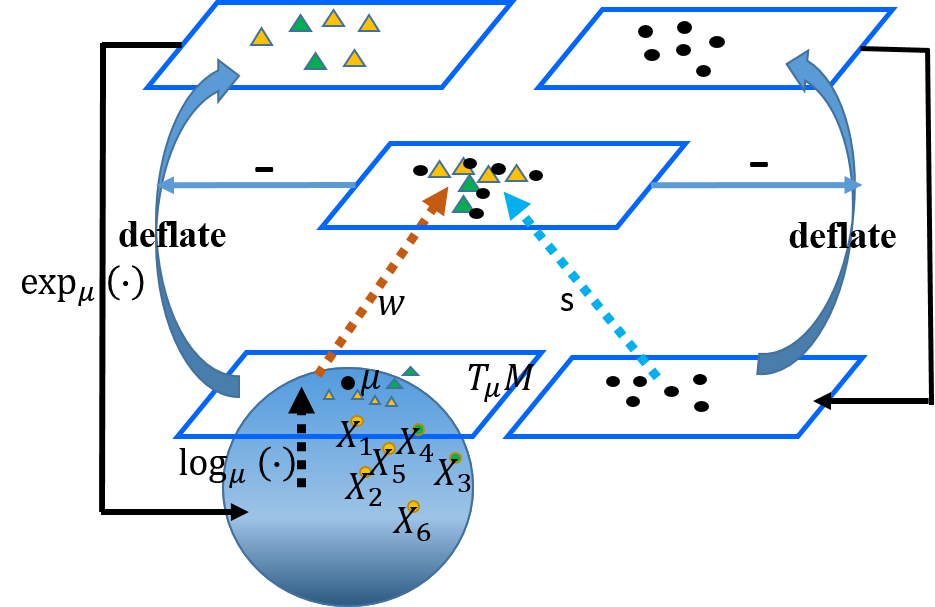
\includegraphics[width=0.7\linewidth]{source/multi_discrim_tangent_PLS.png}
	\caption{算法\ref{alg:RPLS_multi_support_approx_regression}的示意图}
	\label{fig:multi_discrim_tangent_PLS}
\end{figure}

在训练数据上运用算法\ref{alg:RPLS_multi_support_approx_regression}的到训练参数后,测试的部分与普通的算法\ref{alg:RPLS_discrim_tangent_approx_regression}或\ref{alg:RPLS_approx_regression}的测试类似,所不同的是算法\ref{alg:RPLS_multi_support_approx_regression}中回归的$Y$是所有切空间中结果的综合(逐步回归相加)得到的。

关于训练,算法\ref{alg:RPLS_multi_support_approx_regression}与\ref{alg:RPLS_discrim_tangent_approx_regression}和\ref{alg:RPLS_approx_regression}有些许的不同:首先是算法\ref{alg:RPLS_multi_support_approx_regression}的参数$k$的选择往往要比后两者的小很多,例如在YTC\cite{Database_YTC}数据集上算法\ref{alg:RPLS_approx_regression}和\ref{alg:RPLS_discrim_tangent_approx_regression}的参数$k$默认设置为类别数减一(46=47-1)且实验发现减小$k$会使得算法的性能降低,而算法\ref{alg:RPLS_multi_support_approx_regression}中$k$的选择为26,过高或过低都会降低算法的性能(原因可能是欠拟合或过拟合了);算法\ref{alg:RPLS_multi_support_approx_regression}的另一个重要的参数的选择就是$p$,这个也会有欠拟合和过拟合的现象;最后是在测试的时候发现,数据是否中心化对算的最终结果也有一定的影响,这个问题在UIUC\cite{Database_UIUC}数据上做材料分类的时候尤其明显。
\section{实验验证}
\label{sec:RPLS_exp}
前面的章节对问题的背景,已有的方法,存在的问题以及本文的动机和针对问题的解决的方案等做了阐述,本节将会实验验证前面的方法并从实验结果出发分析方法的特点和存在的问题等。

本实验主要从以下几个计算机视觉的任务进行验证:物体识别(数据库ETH80\cite{Database_ETH80}),材料分类(数据库UIUC\cite{Database_UIUC})以及视频人脸识别(数据集YTC\cite{Database_YTC});由于这些数据集已经在\ref{sec:data_intro}节进行了介绍,并且这些数据集的测试协议也已经在\ref{sec:data_intro}节中介绍,所以这里就不再进行阐述,如果读者对数据或测试协议有什么不明的话可以到\ref{sec:data_intro}一节进行查看。
\subsection{原始特征构造}
\label{Database_feature}
这里将简单的介绍一下,各个任务对应的数据集上的基本特征的构造,这些特征底层特征的提取将用于最后的SPD矩阵(实际上也可看作是一种特征表示)的构造。首先,在用于物体识别的ETH80\cite{Database_ETH80}数据集上,所有的图片被预先被resize成$20\times 20$的大小图片,然后灰度特征被直接用于物体识别任务;在材料识别任务的UIUC\cite{Database_UIUC}数据集上,这里使用Region Covariance\cite{RegionCov}表示一张图片,参考\cite{Statistics_SPDML},这里的Region Covariance 的构造中我们使用128维的dense SIFT\cite{SIFT}特征作为基本的特征:首先将图片resize到$400\times400$然后,以4个像素为间隔(每个块的大小为$16 \times 16$,共8个角度,4个bin)划分网格,在每个网格点128维的SIFT特征被提取作为构造Region Covariance的基本特征(与工作\cite{Statistics_SPDML}中的不同的是工作\cite{Statistics_SPDML}还融合了颜色特征);最后在视频人脸识别任务的数据库YTC\cite{Database_YTC}上,首先将图片resize到$20\times 20$然后直方图均衡化被用于鲁棒的特征构造。
\subsection{对称正定矩阵表示的构造}
\label{sec:Database_SPD_Construct}
在“原始特征构造\ref{Database_feature}”这一小节介绍了基本的图像特征的提取和预处理方式,在本节中将对使用这些基本特征构造SPD矩阵表示做简要的介绍:首先是材料识别任务的UIUC\cite{Database_UIUC}数据集上的SPD表示,由于使用的是Region Covariance\cite{RegionCov},这里使用的是标准的构造方式,故不再做进一步介绍,有兴趣的读者可以参看文献\cite{RegionCov};在物体识别的ETH80\cite{Database_ETH80}和视频人脸识别的\cite{Database_YTC}数据集上,这里根据工作\cite{Statistics_CDL}中的内容使用SPD矩阵表示图像集合,但是稍微有些不同的是:根据\cite{Statistics_HERML,Statistics_DARG}中的构造方式,均值的信息也被融入了图像集合的SPD特征表示当中(公式\ref{MeanCov_SPD_Construct}中的$\Sigma$是样本协方差,$\bm{m}$是样本均值,$d$是样本的维数):
\begin{equation}
\label{MeanCov_SPD_Construct}
C={\rm det}(\Sigma)^{-\frac{1}{d+1}}\left[
\begin{array}{cc}
\Sigma+\bm{m}\bm{m}^{T}&m\\
\bm{m}&1
\end{array}
\right]
\end{equation}
最后还需要一提的是对于所有的原始特征实验中都做了$95\%$的PCA降维处理;对于样本协方差矩阵$\Sigma$奇异的时候(往往是由于样本个数小于样本维度造成的),根据\cite{Statistics_DARG,Statistics_LEML}中的做法,一个小的正的正则项:$\delta\bm{I},\delta=10^{-3}\times {\rm tr}(C)$(其中$\bm{I}$是单位阵)被加到$\Sigma$上:$\Sigma+\delta\bm{I}\rightarrow \Sigma$。
\subsection{实验结果与分析}
\label{sec:RPLS_exp_result_analysis}
在本实验中,我们将本文所提的方法统一用缩写RPLS(Riemannian Partial Least Squear regression,黎曼偏最小二乘方法)表示,本小结的内容是RPLS方法在物体识别,材料识别以及视频人脸识别三个任务上的实验结果呈现,在对比方法中我们选取了具有代表性的方法:基于PLS的协方差判别学习方法(Covariance Discriminant Learning,CDL)\cite{Statistics_CDL},黎曼稀疏编码学习的方法(Riemannian Sparse Representation,RSR),然后是发表在2014年欧洲计算机视觉会议(European Conference On Computer Vision,ECCV)上的工作:对称正定矩阵流形学习(SPD-Manifold Learning,SPDML)在两种度量(Stein Divergence\cite{Stein_divergence}和Affine Invariant Metric\cite{AIM_metric})下的方法,以及使用分布函数建模集合的方法DARG\cite{Statistics_DARG}和BeyondGauss\cite{Statistics_BeyondGauss}以及SPD矩阵流形上的度量学习(Metric Learning)方法LEML\cite{Statistics_LEML}。表\ref{tab:RPLS_experiment}给出了这些方法在三个任务上的实验对比结果,其中所有的结果均是按照\ref{sec:data_intro}节的协议获得的,对于其它文章的方法,这里从作者的主页上获得源代码并小心的调整参数后报告的是在\ref{sec:data_intro}节的协议下所获得的最好的结果。
\begin{table}[htb]
	\centering
	\caption{黎曼流形上的PLS回归算法实验结果}
	\begin{tabular*}{\linewidth}{@{\extracolsep{\fill}}|l|ccc|}\hline
		\diagbox{方法}{数据集} &ETH80 &UIUC &YTC \\ \hline
		CDL-PLS\cite{Statistics_CDL} &93.25$\pm$4.72 &53.89$\pm$4.06 &70.28$\pm$2.13 \\ \hline
		RSR-Stein\cite{Dictionary_RSR} &93.25$\pm$3.34 &52.41$\pm$4.03 &72.77$\pm$2.69  \\ \hline
		SPDML-Stein\cite{Statistics_SPDML} &90.50$\pm$3.87 &49.17$\pm$2.37 &61.57$\pm$3.43  \\ \hline
		SPDML-AIM\cite{Statistics_SPDML} &90.75$\pm$3.34 &48.09$\pm$1.82 &64.66$\pm$2.92  \\ \hline
		BeyondGauss\cite{Statistics_BeyondGauss} &84.75$\pm$6.29 &N/A &71.46$\pm$2.61  \\ \hline
		DARG\cite{Statistics_DARG} &92.25$\pm$2.19 &N/A &77.09$\pm$1.92  \\ \hline
		LEML\cite{Statistics_LEML}&94.75$\pm$2.49 &48.98$\pm$3.69 &70.53$\pm$2.95  \\ \hline
		$\rm \bm{RPLS_{single}}$ &\textbf{92.75$\pm$4.32} &\textbf{54.72$\pm$3.61} &\textbf{74.48$\pm$2.79}  \\ \hline
		$\rm \bm{RPLS_{multi}}$ &\textbf{95.50$\pm$2.58} &\textbf{56.57$\pm$3.49} &\textbf{77.33$\pm$2.95}  \\ \hline
	\end{tabular*}
	\label{tab:RPLS_experiment}
\end{table}

其中,$\rm RPLS$算法的下标表示的基础版本的黎曼流形上的PLS算法\ref{alg:RPLS_discrim_tangent_approx_regression}($\rm \bm{RPLS_{single}}$)还是多切空间逐步回归的算法\ref{alg:RPLS_multi_support_approx_regression}($\rm \bm{RPLS_{multi}}$)。最终的实验结果验证了我们最初的猜想,多切空间偏最小二乘回归算法在三个任务上都获得了state-of-the-art的结果;我们将取得这样的结果的原因归结为(与CDL\cite{Statistics_CDL}相比):1)首先是按照公式\ref{MeanCov_SPD_Construct}构造的SPD表示中均值信息者带来了一定性能上的提升;2)考虑切空间的选择带来了表格倒数第二行和表格第一行的变化(因为CDL-PLS与在单位阵切空间中的$\rm \bm{RPLS_{single}}$是等价的);3)最后是单切空间与多切空间的方案差别带来了表格中最后两行的变化,同时也力证多切空间逐步回归算法\ref{alg:RPLS_multi_support_approx_regression}的有效性。

试验中我们发现公式\ref{support_search}中的第二项对算法性能有小幅的提升,试验中我们始终固定公式中$\lambda=0.001$。而在前面我们也有介绍,算法\ref{alg:RPLS_multi_support_approx_regression}中的参数$k,p$对于算法的影响较大,也是本算法需要改进的一大方向。

最后在对比的一系列的方法中,BeyondGauss\cite{Statistics_BeyondGauss}的方法由于是使用KDE来估计分布函数,而在UIUC\cite{Database_UIUC}这个数据集上原始的特征是Dense Sift(样本非常多),直接导致了无法计算的问题,所以这里的结果没有汇报(N/A),其它的结果是在hellinger散度下的结果。同样由于内存问题GARG方法在UIUC数据集上也无法获得结果,所以也使用N/A代替。表格中对比方法的结果都是从作者主页获取的代码小心调参后获得的最好的结果。
\section{总结与下一步工作}
\label{sec:conclusion_futurework}
本章从子流形与投影的概念出发,参考相关工作\cite{PGA,RCCA,AIM_metric,Statistics_CDL}等首先导出了黎曼流形上的偏最小二乘问题以及偏最小二乘用于回归的一般形式,然后以SPD矩阵流形为例将算法形式化到\ref{alg:RPLS_approx_regression}中,并针对图像集合分类问题与DTI(Diffusion Tensor Images)的不同(主要是数据更稀疏的问题),提出了两点通用的改进(这里之所以说是通用的改进,是因为即便数据聚集在流形的小范围内这些改进依然是适用的)得到了多切空间偏最小二乘回归算法,使得算法可以适应这种数据稀疏的情况,最后的实验验证部分验证了方法的有效性。

实验分析部分以及算法\ref{alg:RPLS_multi_support_approx_regression}分析部分都提到,算法\ref{alg:RPLS_multi_support_approx_regression}中的参数$k,p$太大会过拟合太小又会欠拟合,分析其原因的话可能是逐步回归的方式没能有效的组合各个切空间中的信息,接下来可能参考\cite{RegionCov_pedestrain}中的方法使用Adaboost的框架进行多个切空间中模型的组合。